\documentclass[
% preprint,
% preprintnumbers,
 amsmath,amssymb,
 aps,
 pre,
 longbibliography,
 10pt, onecolumn,
 notitlepage
]{revtex4-1}


\usepackage{graphicx}% Include figure files
\graphicspath{{./figures/}} % path to figures
\usepackage{dcolumn}% Align table columns on decimal point
\usepackage{bm}% bold math
\usepackage{hyperref}% add hypertext capabilities
\usepackage{physics} % package for physics symbols

% for referencing main.tex (c.f. xr-package example)
\usepackage{xr}
\makeatletter
\newcommand*{\addFileDependency}[1]{% argument=file name and extension
  \typeout{(#1)}
  \@addtofilelist{#1}
  \IfFileExists{#1}{}{\typeout{No file #1.}}
}
\makeatother

\newcommand*{\myexternaldocument}[1]{%
    \externaldocument{#1}%
    \addFileDependency{#1.tex}%
    \addFileDependency{#1.aux}%
}
\myexternaldocument{main}


\begin{document}
% define commands
\newcommand{\eqnname}{Eqn.}
\newcommand{\secname}{Sec.}
% adding S prefix
\renewcommand{\theequation}{S\arabic{equation}}
\renewcommand{\thefigure}{S\arabic{figure}}
\renewcommand{\bibnumfmt}[1]{[S#1]}
\renewcommand{\citenumfont}[1]{S#1}

\title{Supplemental Material}

\author{empty}
\affiliation{empty}

\maketitle

This supplemental material contains derivations of main equations in the paper. Derivations include the formula for energy flux \eqnname~\eqref{eqn:flux_def}, linear response theory \eqnname~\eqref{eqnS:response},\eqref{eqn:flux_integral},\eqref{eqn:flux_residue}, eigenmode decomposition \eqnname~\eqref{eqn:flux_eigen}, and path summation \eqnname~\eqref{eqn:flux_path}.

\section{The formula for energy flux}
In this section, we derive the formula for energy flux \eqnname~\eqref{eqn:flux_def}.
Here the force $F$ does not need to be linear, and it is a general conservative force.
The strategy to find the energy flux is that, first define the energy $E_i$ of particle $i$, then write down the infinitesimal energy change $dE_i$ using stochastic calculus, finally identify terms in $dE_i$ that is caused by neighboring particles, and define these terms as the energy transfer among particles.

The energy of particle $i$ is defined as
\begin{equation} \label{eqnS:energy_individual}
E_i = \frac{1}{2}m_iv_i^Tv_i + U_{ii} + \frac{1}{2}\sum_jU_{ij},
\end{equation}
where the first term is the kinetic energy, the second term is the on-site potential, and the last term is one half of spring energy between the particle and its neighbors.

To calculate $dE_i$, we use Ito's formula. Because we need the average of $dE_i$, and the stochastic term in Ito's calculus is non-anticipating, which vanishes under time-average.
For a stochastic differential equation (SDE) of variable $X$ with drift $\mu$ and diffusion $\sigma$
\begin{equation} \label{eqnS:SDE_general}
dX = \mu dt + \sigma dW ,
\end{equation}
Ito's formula gives the SDE of function $f(X)$
\begin{equation} \label{eqnS:SDE_ito}
df(X) = ((\nabla_X^Tf)\mu + \frac{1}{2}\tr[\sigma \sigma^T \nabla_X\nabla_X^Tf])dt + (\nabla_X^Tf) \sigma dW .
\end{equation}

For our system, we can represent $N$ particles by a column vector $z = \sum_{i=1}^N \ket{i}\otimes z_i$, with $\ket{i}$ denoting the 2D subspace of $i$, likewise for $v$ and $\eta$, then we get
\begin{align}
X &= \pmqty{ z & v & \eta }^T, \label{eqnS:SDE_X}\\
\mu &= \pmqty{ v \\
\frac{1}{m}(-\nabla_zU - BAv - \gamma v + \eta) \\
-\frac{1}{\tau}\eta }, \label{eqnS:SDE_mu} \\
\sigma &= \text{diag} \pmqty{0 & 0 & \frac{\sqrt{2\gamma T_a}}{\tau} I}, \label{eqnS:SDE_sigma}
\end{align}
where U is the total energy of the system, $A$ is an antisymmetric matrix $A=\sum_i \ket{i}\bra{i}\otimes \mqty(0 & 1 \\ -1 & 0)$, and $\text{diag}()$ means a block-diagonal matrix.
The function $f(X)$ is the energy of particle $i$, $E_i$.
The nonzero terms in the gradients of $E_i$ are
\begin{align}
\nabla_{z_i}E_i &= -(F_{ii} + \frac{1}{2}\sum_jF_{ji}), \\
\nabla_{z_j}E_i &= -\frac{1}{2}F_{ij}, \\
\nabla_{v_i}E_i &= m_iv_i.
\end{align}

Now we apply Ito's formula \eqnname~\eqref{eqnS:SDE_ito} to our system.
The term $(\nabla_X^TE_i)\mu$ reads
\begin{equation}
\begin{split}
(\nabla_X^TE_i)\mu
&= (\nabla_{z_i}^TE_i)v_i + \sum_j(\nabla_{z_j}^TE_i)v_j + (\nabla_{v_i}^TE_i)m_i^{-1}(-\nabla_{z_i}U - BAv_i - \gamma v_i + \eta_i) \\
&= -(F_{ii} + \frac{1}{2}\sum_jF_{ji})^T v_i - \sum_j\frac{1}{2}F_{ij}^T v_j + v_i^T (F_{ii} + \sum_jF_{ji}) - \gamma v_i^Tv_i + v_i^T\eta_i \\
&= -\sum_j\frac{1}{2}(v_i + v_j)^T F_{ij} - \gamma v_i^Tv_i + v_i^T\eta_i ,
\end{split}
\end{equation}
where we used $F_{ji} = -F_{ij}$ and $v_i^TAv_i = 0$.
The term $\frac{1}{2}\tr[\sigma \sigma^T \nabla_X\nabla_X^Tf]$ and $\nabla_X^Tf$ are zero.

Finally, the energy change can be written as
\begin{align}
dE_i &= -\sum_jJ_{ij}dt + h_i dt, \label{eqnS:flux_dEi} \\
J_{ij} &= \frac{1}{2}(v_i + v_j)^T F_{ij}, \label{eqnS:flux_Jij} \\
h_i &= -\gamma_i v_i^Tv_i +v_i^T\eta_i. \label{eqnS:flux_hi}
\end{align}
In the energy change $dE_i$, the term $J_{ij}$ involves particle $i$ and its neighbors, and $dh_i$ term involves $i$ and the bath. We identify $J_{ij}$ as the heat transferred (per unit time) from particle $i$ to $j$, and $h_i$ as the heat transferred from particle $i$ to the bath.

As for the steady-state average of $J_{ij}$, one can use $\expval{\frac{d}{dt}U_{ij}=0}$ and the chain rule to get the derivative of $U_{ij}$ with respect to positions, i.e. the force
\begin{equation}
    0 = v_i^T F_{ji} + v_j^T F_{ij}
    = -v_i^T F_{ij} + v_j^T F_{ij},
\end{equation}
and arrive at a reduced expresion
\begin{equation}
    \expval{J_{ij}} = \expval{v_j^T F_{ij}}.
\end{equation}


\section{Algebraic method for solving the energy flux}
One straightforward method to compute the flux $J$ is as follows.
A system is determined by the network geometry and parameters $m, k_g, k, B, \gamma, \tau, T_a$.
Given the equation of motion \eqnname~\eqref{eqnS:SDE_general},\eqref{eqnS:SDE_X}-\eqref{eqnS:SDE_sigma}, one can numerically solve for the covariance $C=\expval{XX^T}$ from the matrix equation $\mu C + C \mu^T = \sigma\sigma^T$ \cite{Gardiner2009ItoCalculus,Ceriotti2010ColoredNoiseThermostats}.
Finally, the flux \eqnname~\eqref{eqnS:flux_Jij}, which is bilinear in $x$ and $v$, can be extracted from the covariance $C$.


\section{Energy flux from linear response theory}
Following \cite{Kundu2011LargeDeviations}, we calculate the energy flux using linear response theory, which expresses the flux by the response function.
We first arrive at the response function \eqnname~\eqref{eqnS:response}, then get a raw expression of flux using the response function \eqnname~\eqref{eqnS:flux_integral_raw}, finally simplify this expression and get \eqnname~\eqref{eqn:flux_integral} and \eqref{eqn:flux_residue} in the paper.
After the derivation there will be some discussions on the result.

We define Fourier transform (FT) as below
\begin{align}
\tilde{f}(\omega) &= \frac{1}{t} \int_0^t dt'\ f(t')e^{-i\omega t'},\quad
\omega = \frac{2\pi n}{t} ,\\
f(t) &= \sum_{\omega=-\infty}^{\infty} \tilde{f}(\omega) e^{i\omega t} .
\end{align}

From the equation of motion \eqnname~\eqref{eqnS:SDE_general},\eqref{eqnS:SDE_X}-\eqref{eqnS:SDE_sigma}, one can write down the FT of the whole system
\begin{align}
\tilde{v}(\omega) &= i\omega \tilde{z}(\omega) ,\label{eqnS:FT_v}\\
\tilde{z}(\omega) &= G^+(\omega) \tilde{\eta}(\omega) ,\label{eqnS:FT_z}\\
\tilde{\eta}(\omega) &= \frac{\sqrt{2\gamma T_a}}{1 + i\omega \tau} \tilde{\xi}(\omega) ,\label{eqnS:FT_eta}
\end{align}
where $G^+$ is the response function is defined as
\begin{equation} \label{eqnS:response}
G^{\pm}(\omega) = [K \pm i\omega(\gamma I + BA) - m\omega^2I]^{-1} .
\end{equation}

Now we turn to the heat flow.
Since $J(t')$ has a bilinear form, its time integral $Q = \int_0^t \dd{t'} J(t')$ can be written as a sum of Fourier modes using Parseval's theorem,
\begin{equation} \label{eqnS:qmode_sum}
Q = t\sum_{\omega=-\infty}^{\infty} \tilde{q}_\omega
\overset{\tilde{q}_0 = 0}{=}  t\sum_{\omega=2\pi/t}^{\infty} (\tilde{q}_\omega + \tilde{q}_{-\omega}) .
\end{equation}
To calculate the mode $\tilde{q}_\omega$, we need to express $J_{ij}$ in $z$ instead of $F$, and the result is
\begin{align}
J_{ij} &= kv^TA^{J}z \\
\begin{split}
A^{J} &\equiv \frac{1}{2} (\ket{i}\bra{i} \otimes e_{ij}e_{ij}^T + \ket{i}\bra{j} \otimes e_{ij}e_{ji}^T \\
&\quad + \ket{j}\bra{i} \otimes (-e_{ji}e_{ij}^T) + \ket{j}\bra{j} \otimes (-e_{ji}e_{ji}^T)) .
\end{split}
\end{align}
The Fourier modes of heat $q_\omega$ and its conjugate $q_{-\omega}$ read
\begin{align}
q_\omega &= k\tilde{v}^T A^{J} \tilde{z}^*
= i\omega k \tilde{\eta}^TG^{+T}A^{J}G^-\tilde{\eta}^* ,\\
q_{-\omega} &= -i\omega \tilde{\eta}^\dagger G^{-T}A^{J}G^+\tilde{\eta}
= -i\omega \tilde{\eta}^TG^{+T}{A^{J}}^TG^-\tilde{\eta}^* .
\end{align}
Adding $q_\omega$ and $q_{-\omega}$ to get $A_\omega^q$,
\begin{align}
\tilde{q}_\omega + \tilde{q}_{-\omega} &= \tilde{\eta}(\omega)^T A_\omega^q \tilde{\eta}(\omega)^* \\
A_\omega^q &= -i\omega k G^{+T}(\omega) A^{as} G^-(\omega), \\
A^{as} &= -(A^{J} - {A^{J}}^T)
= -\ket{i}\bra{j} \otimes e_{ij}e_{ji}^T + \ket{j}\bra{i} \otimes e_{ji}e_{ij}^T .
\end{align}

Averaging $\tilde{q}_\omega + \tilde{q}_{-\omega}$ over the noise $\tilde{\eta}(\omega)$ using the relationship between $\tilde{\eta}$ and $\tilde{\xi}$ \eqnname~\eqref{eqnS:FT_eta}, and $\expval{\tilde{\xi}(\omega) \tilde{\xi}^T(\omega')} = \frac{1}{t} I \delta(\omega + \omega')$, one gets
\begin{equation} \label{eqnS:qmode_single}
\begin{split}
\expval{\tilde{q}_\omega + \tilde{q}_{-\omega}}
&= \frac{2\gamma T_a}{1 + \omega^2 \tau^2} \tr[A_\omega^q \expval{\tilde{\xi}(-\omega)\tilde{\xi}(\omega)^T}] \\
&= \frac{1}{t} \frac{2\gamma T_a}{1 + \omega^2 \tau^2} \tr A_\omega^q .
\end{split}
\end{equation}

In long time limit, the sum can be approximated by an integral
\begin{equation}
\frac{1}{t} \sum_{\omega=2\pi/t}^{\infty}
= \frac{1}{2t} \sum_{\omega=-\infty}^{\infty} \frac{t \Delta\omega}{2\pi}
\approx \frac{1}{4\pi}\int_{-\infty}^{\infty} \dd{\omega} .
\end{equation}
Using this integral conversion, \eqnname~\eqref{eqnS:qmode_sum} and \eqref{eqnS:qmode_single} can be turned to a raw formula for the flux
\begin{equation} \label{eqnS:flux_integral_raw}
\expval{J} = \lim_{t\rightarrow \infty} \frac{\expval{Q}}{t}
= \frac{\gamma T_a}{2\pi} \int_{-\infty}^{\infty} \dd{\omega} \frac{\tr A_\omega^q}{1+\omega^2\tau^2} .
\end{equation}

In the final step, we simplify this integral with the help of the property \cite{Kundu2011LargeDeviations}
\begin{equation} \label{eqnS:response_property}
G^-(\omega) - G^{+T}(\omega) = 2i\omega\gamma G^-(\omega)G^{+T}(\omega) .
\end{equation}
Using this property, the trace of $A_\omega^q$ becomes
\begin{equation}
\begin{split}
\tr A_\omega^q &= -i\omega k \tr G^{+T} A^{as} G^- \\
&= -i\omega k \frac{1}{2i\omega \gamma} \tr (G^- - G^{+T})A^{as} \\
&= -\frac{k}{2\gamma} (\tr G^-A^{as} - \tr G^{+T}A^{as}) \\
&= -\frac{k}{\gamma} \Re\tr G^+A^{as} .
\end{split}
\end{equation}

Plugging this trace into \eqnname~\eqref{eqnS:flux_integral_raw}, we get the integral form for the flux \eqnname~\eqref{eqn:flux_integral}
\begin{equation}
\expval{J} = -\frac{T_ak}{2\pi} \int_{-\infty}^{\infty} \dd{\omega} \frac{\Re \tr G^+A^{as}}{1+\omega^2\tau^2} .
\end{equation}

This integral form can be further simplified using residue theorem.
Since $\Im G^+(-\omega) = -\Im G^+(\omega)$,
$\frac{\Im \tr G^+A^{as}}{1+\omega^t\tau^2}$ is an odd function of
$\omega$, and its line integral vanishes.
\begin{equation}
\expval{J} = -\frac{T_ak}{2\pi} \int_{-\infty}^{\infty} \dd{\omega} \frac{\tr G^+A^{as}}{1+\omega^2\tau^2} .
\end{equation}
The integrand vanishes at $\omega \rightarrow \infty$, so the line
integral can be converted to a contour integral along the
counter-clockwise semicircle $R$ in the lower-half plane
\begin{equation}
\expval{J} = \frac{T_ak}{2\pi} \oint_R \dd{\omega} \frac{\tr G^+A^{as}}{1+\omega^2\tau^2} .
\end{equation}
The noise correlation $\tau$ introduces a pole of the integrand at $\omega=-i/\tau$, thus the contour integral can be evaluated as
\begin{equation} \label{eqnS:flux_residue}
\expval{J} = -\frac{T_ak}{2\tau} \tr G^+(-\frac{i}{\tau})A^{J,as} ,
\end{equation}
and the response function at $-i/\tau$ reads
\begin{equation} \label{eqnS:response_at_pole}
G^+(-\frac{i}{\tau})
= [K + (\frac{\gamma}{\tau} + \frac{m}{\tau^2})I + \frac{B}{\tau}A]^{-1} .
\end{equation}

In theory, the equation \eqnname~\eqref{eqnS:flux_residue} provides the analytical solution of the flux, because the inverse matrix \eqnname~\eqref{eqnS:response_at_pole} can be expressed analytically.
In practice, analytical solutions can be easily calculated for small networks, but hard for large networks.
Nevertheless, one can obtain some general properties of the flux from \eqnname~\eqref{eqnS:flux_residue} after some algebra. For network with only horizontal and vertical bonds (as in \figurename~\ref{fig:model_and_result}d), all fluxes are zero. For two networks whose slanted bonds have opposite angles (as in \figurename~\ref{fig:model_and_result}c and e), their fluxes are opposite. Changing $B$ to $-B$ would change the flux $J$ to $-J$.


\section{Kirchoff's law}
The derivation of the Kirchoff's law is similar to the derivation of the energy flux, except that we use the heat from particle to the bath $h_i$ in \eqnname~\eqref{eqnS:flux_hi} instead of $J_{ij}$ in \eqnname~\eqref{eqnS:flux_Jij}.

Following the procedure in the last section from \eqnname~\eqref{eqnS:qmode_sum} to \eqref{eqnS:flux_integral_raw}, we arrive at a raw formula for the flux $\expval{h_i} = \frac{\gamma T_a}{2\pi} \int_{-\infty}^{\infty} \dd{\omega} \frac{\tr A_\omega^q}{1+\omega^2\tau^2}$ with a different $A_\omega^q$ for $h_i$
\begin{gather}
A_\omega^q = i\omega (G^{+T} \rho_i - \rho_iG^-) - 2\gamma\omega^2 G^{+T} \rho_i G^- ,\\
\rho_i = \ket{i}\bra{i} .
\end{gather}

Using the property of $G^\pm$ \eqnname~\eqref{eqnS:response_property}, one gets
\begin{equation}
\begin{split}
\tr (G^{+T} \rho_i - \rho_iG^-)
&= \tr \rho_i(G^{+T} - G^-) \\
&= -\tr \rho_i 2i\omega \gamma G^- G^{+T} \\
&= -2i\omega\gamma \tr G^{+T}\rho_i G^- ,
\end{split}
\end{equation}
so the trace of $A_\omega^q$ vanishes
\begin{equation}
\tr A_\omega^q
= i\omega \tr (G^{+T} \rho_i - \rho_iG^-) - \tr 2\gamma\omega^2 G^{+T} \rho_i G^-
= 0 .
\end{equation}
This means that $\expval{h_i}$ is also zero, so on average there is no heat exchange between the particle and the bath. Since the average change of $E_i$ is zero, and $\expval{\dot{E_i}} = -\sum_j\expval{J_{ij}} + \expval{h_i}$, we get the Kirchoff's law
\begin{equation}
    -\sum_j\expval{J_{ij}} = \sum_j\expval{J_{ji}} = 0 .
\end{equation}


\section{Connection to isolated gyroscopic networks}

\begin{figure}[ht]
	\centering
	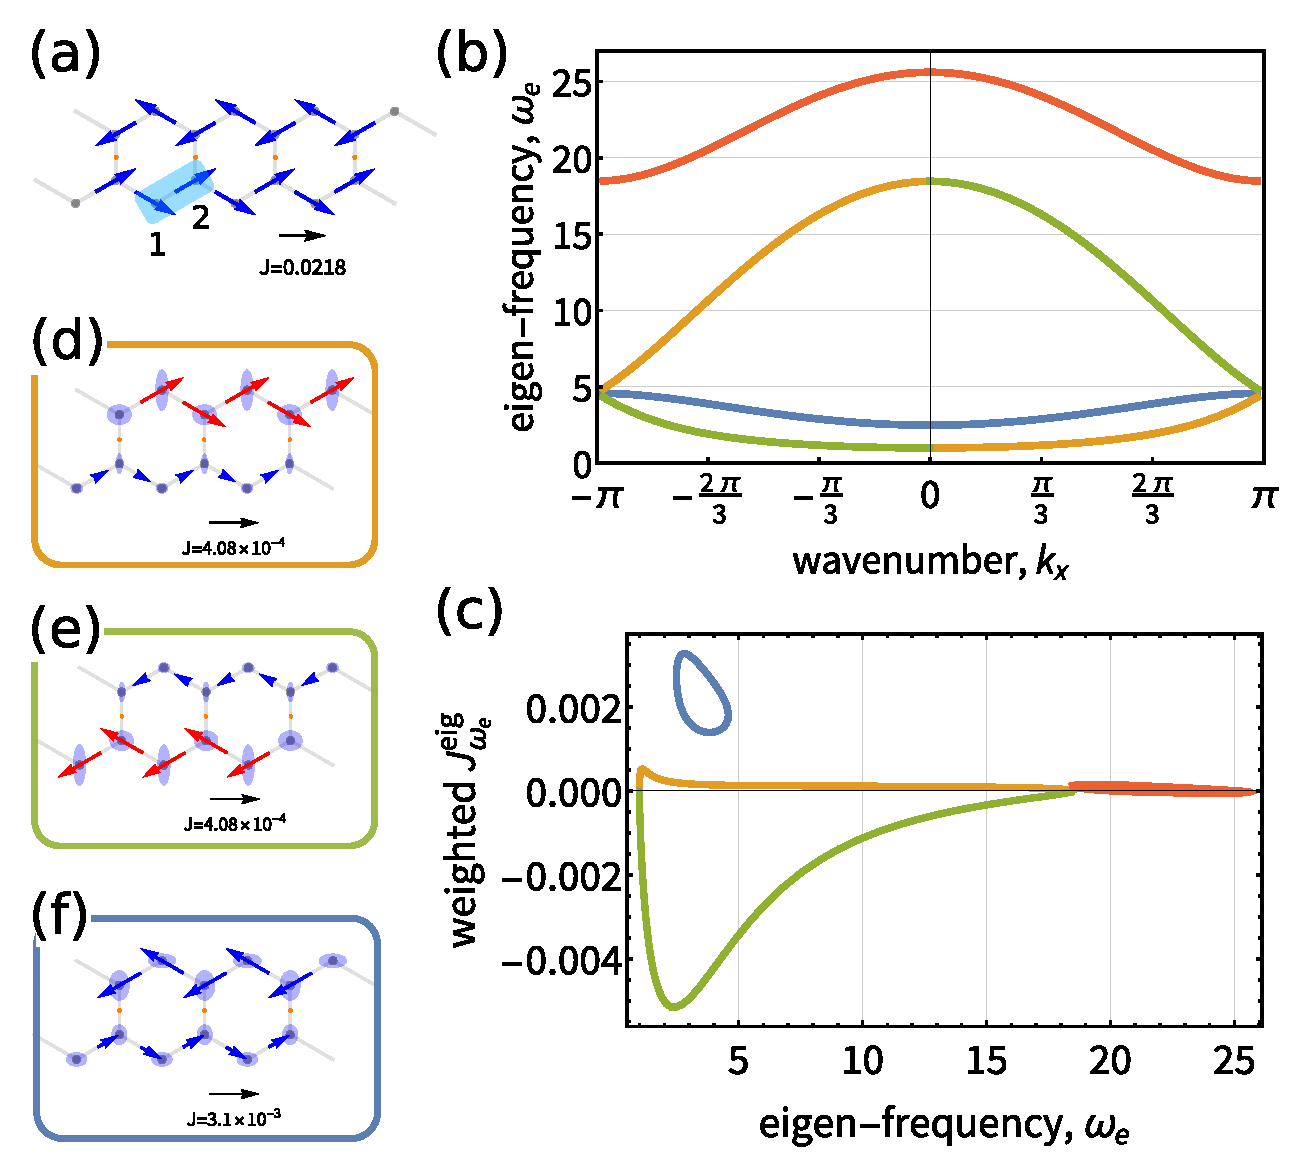
\includegraphics[width=0.45\textwidth]{3_eigen_modes.pdf}
    \caption{Using the eigenmode decomposition, we explain how the flux in honeycomb network is CCW, even though its edgemodes contribute to CW flux.
    (a) Network used for calculation, which consists of one row of hexagons (51 unit cells) and has periodic boundary in $x$ direction. Parameters: $k_{g,\tau}=1, k=10$, others are $1$.
    (b) Band structure of the network (marked with different colors). The yellow/green band contains CW flux localized on the top/bottom edge (an example mode is shown in (d)/(e)). The blue band contains bulk modes with CCW flux (also see (f)).
    (c) Weighted flux $J_{\omega_e}^{eig}$ from $1$ to $2$ (marked in (a)) of the four bands. Total flux in the green band with CW edge modes and the blue band with CCW bulk modes are $-0.106$ and $0.115$, respectively. As a result, the net flux is CCW.
    }
    \label{fig:eigen_modes}
\end{figure}

Since our model is built upon the well-studied isolated system \cite{Nash2015TopologicalMechanics,Susstrunk2016ClassificationTopological,Mitchell2018AmorphousTopological,Lee2018TopologicalDynamics}, we would like to build a connection between our energy flux in the active system and eigenmodes in those studies.
In this section, we show that the flux formula \eqnname~\eqref{eqn:flux_residue} can be decomposed to a weighted sum over eigenmodes \eqnname~\eqref{eqn:flux_eigen}. Then we apply this result to a honeycomb network as an example.

For clarification, the Fourier analysis from \secname~\ref{sec:fourier} in the main text is not suitable for this connection, because Fourier modes and eigenmodes are related only at small $\gamma$'s (\figurename~\ref{fig:Fourier_modes}b and c), but they become dissimilar at larger $\gamma$'s (\figurename~\ref{fig:Fourier_modes}b and d).
The underlying discrepancy between Fourier modes and eigenmodes is that, eigenmodes are for the isolated network, whereas Fourier modes have an extra factor of friction or damping.
In addition to this extra factor $\gamma$,
the active system also has extra factors of $m$ and $\tau$. The factor $m$ comes from the order of dynamics: the active system is $2$nd order in time, while the gyroscopic dynamics in \cite{Nash2015TopologicalMechanics} is $1$st order, which corresponds to the $m\rightarrow 0$ limit.

Our starting point is \eqnname~\eqref{eqn:flux_residue}. The key bridge for these gaps is that, in $G^+(-i/\tau)$ from the equation, $\gamma,m,\tau$ are not independent factors, they act collectively through $k_{g,\tau} \equiv k_g+\frac{\gamma}{\tau}+\frac{m}{\tau^2}$, so the extra factors $m,\gamma, \tau$ only add a modification to $k_g$.
We let the reference isolated system we connect to have a modified on-site spring constant $k_{g,\tau}$, then after some algebra, one can show that the flux $\expval{J}$ in active system can be written as a weighted sum of the flux of each eigenmode $J^{\text{eig}}_{\omega_e}$ in the reference system (for its derivation, see the next section),
\begin{equation} \label{eqn:flux_eigen}
    \expval{J} = \sum_{\omega_e} \frac{1}{1+\omega_e^2\tau^2} J^{\text{eig}}_{\omega_e}.
\end{equation}
Here $\omega_e$ is the (discrete) eigen-frequency of the reference system, not to be confused with the (continuous) Fourier frequency $\omega$. The amplitude of eigenmode is set such that its energy is $T_a$, and $J^{\text{eig}}_{\omega_e}$ is the time-averaged energy flux.
A related equation is a ``sum rule", the unweighted sum of all modes is zero, $\sum_{\omega_e} J^{\text{eig}}_{\omega_e} = 0$. This can be shown from direct calculations (Supplemental Material).

From this eigenmode decomposition, the discussion of TRS in the isolated system \cite{Nash2015TopologicalMechanics} immediately carries over to the active system. For network geometries that satisfy TRS, the energy flux of eigenmodes are zero, thus through \eqnname~\eqref{eqn:flux_eigen}, the flux in active system is also zero. This result can also be obtained from \eqnname~\eqref{eqn:flux_residue} through some linear algebra.

As an application, we will analyze the flux in the honeycomb network using the eigenmode decomposition and the ``sum rule".
The flux pattern in the active honeycomb network displays CCW flux localized on the boundary (\figurename~\ref{fig:model_and_result}f). This localization is reminiscent of the edgemode in \cite{Nash2015TopologicalMechanics} (\figurename~\ref{fig:Fourier_modes}b), however, their directions are opposite.
From the decomposition \eqnname~\eqref{eqn:flux_eigen}, the edgemodes should contribute a large CW flux in the active system, but somewhat surprisingly, the net flux is CCW.
To better analyze the contribution from each eigenmode, we look at a simple honeycomb lattice with only one layer (\figurename~\ref{fig:eigen_modes}a).
This lattice has four bands (\figurename~\ref{fig:eigen_modes}b), two bulk bands (blue, red) and two edge bands (green, yellow). The weighted flux of each band is plotted in \figurename~\ref{fig:eigen_modes}c. We see that the CW edge band does contribute a large CW flux (green curve in \figurename~\ref{fig:eigen_modes}c), however, due to the ``sum rule", the unweighted sum of other bands has to be CCW. In the honeycomb lattice, it happens that many of this CCW fluxes are contained in the lower bulk band (blue curve in \figurename~\ref{fig:eigen_modes}c and example mode in \figurename~\ref{fig:eigen_modes}f). When the flux gets weighted, the CCW flux from lower bulk band outweighs CW flux from the edgemodes, the other two bands (yellow and red curve in \figurename~\ref{fig:eigen_modes}c) also contribute to CCW flux, although relatively small. As a result, the net flux is CCW, which is opposite to the flux of the edgemode.


\section{Derivation of eigenmode decomposition of energy flux}
In deriving the eigenmode decomposition \eqnname~\eqref{eqn:flux_eigen}, we first look at the reference isolated system, write down its eigenmodes \eqnname~\eqref{eqnS:mode_zct} and time-averaged energy flux \eqnname~\eqref{eqnS:mode_J_isolated}, then turn to the active system and decompose the flux \eqnname~\eqref{eqnS:flux_residue} using the eigenmodes to get \eqnname~\eqref{eqnS:mode_J_active}, finally show that the flux from these two sides are actually related in \eqnname~\eqref{eqnS:mode_J_relation}.
Lastly we also derive the ``sum rule" \eqnname~\eqref{eqnS:mode_J_sum}.

\subsection{Reference isolated system}
The reference isolated system has $1$st-order gyroscopic dynamics as in \cite{Nash2015TopologicalMechanics}. In the setup with Lorentz force, the dynamical equation can be obtained by setting the mass to zero, and replacing the force matrix $K$ by $K^\tau \equiv K + (\frac{\gamma}{\tau} + \frac{m}{\tau^2})I$
\begin{equation}
    \dot{z} = \frac{1}{B} A K^\tau z.
\end{equation}
Following \cite{Nash2015TopologicalMechanics}, we convert to complex representation with $z^c \equiv \pmqty{x + iy & x - iy}^T$
\begin{equation}
i \dot{z}^c = \Omega z^c,\quad
K^\tau = i B A O^{-1} \Omega O
\end{equation}
where $O,O^{-1}$ are the transformations between $z$ and $z^c$ $z^c = Oz, z = O^{-1}z^c$.

Writing the eigenvalue problem as
\begin{equation}
\Omega u_{\omega_e} = \omega_e u_{\omega_e} ,
\end{equation}
then the eigenmode with eigen-frequency $\omega_e$ reads
\begin{equation} \label{eqnS:mode_zct}
z^c_{\omega_e}(t) =  (u_{\omega_e} e^{-i\omega_e t} + u_{-\omega_e} e^{i\omega_e t})z_0 ,
\end{equation}
where $z_0$ is the amplitude, and it will be specified shortly.
The eigenmode needs a combination of $\omega_e$ and $-\omega_e$ such that the motion of $x$ and $y$ is real-valued.
This combination is possible because of a symmetry in this eigenvalue problem, when there is $\omega_e$, there is also solution $-\omega_e$ with $u_{-\omega_e} = \pmqty{ 0 & I \\ I & 0 } u_{\omega_e}^*$.

A related property we need later is that, the left eigenvector $v_{\omega_e}$ can be expressed as $v_{\omega_e} = c_{\omega_e} \pmqty{ -I & 0 \\ 0 & I } u_{\omega_e}$,
where $c_{\omega_e}$ is a real prefactor to ensure normalization $v_{\omega_e}^T u_{\omega_e} = 1$.
If there are degenerate eigenvectors (like $v_{\omega_e}^{1},v_{\omega_e}^{2},\dots$), we choose an orthonormal basis set, i.e. $v_{\omega_e}^{i,T} u_{\omega_e}^{j} = 0$ for $i \neq j$.
With the introduction of $c_{\omega_e}$, we now set the amplitude $z_0$ to
$z_0^2 = -\frac{2 c_{\omega_e} T_a}{\omega_e B}$, such that the energy of the eigenmode is $T_a$.

The instantaneous energy flux $J_{\omega_e}$ of mode $z^c_{\omega_e}$ writes
\begin{equation}
\begin{split}
J_{\omega_e} &= (O^{-1} v^{c}_{\omega_e})^T A^J O^{-1}z^c_{\omega_e} \\
&= \tr O^{-1,T} A^J O^{-1}z^c_{\omega_e} v^{cT}_{\omega_e} .
\end{split}
\end{equation}
From the expression of mode \eqnname~\eqref{eqnS:mode_zct},
\begin{equation}
z^c_{\omega_e} v^{cT}_{\omega_e} = -i\omega_e(u_{\omega_e} e^{-i\omega_e t} + u_{-\omega_e}e^{i\omega_e t})(u_{\omega_e}^T e^{-i\omega_e t} - u_{-\omega_e}^Te^{i\omega_e t})z_0^2 .
\end{equation}
When averaging over time, terms like $e^{\pm 2i\omega_e t}$ vanish, so we get
\begin{equation}
\overline{z^c_{\omega_e} v^{cT}_{\omega_e}} = i\omega_e(u_{\omega_e} u_{-\omega_e}^T - u_{-\omega_e} u_{\omega_e}^T)z_0^2 .
\end{equation}
Plugging in $z_0^2 = -\frac{2c_{\omega_e} T_a}{\omega_e B}$, the time-averaged flux of the eigenmode $J_{\omega_e}^\text{eig}$ reads
\begin{equation} \label{eqnS:mode_J_isolated}
J_{\omega_e}^\text{eig} = -\frac{2T_ak}{B} ic_{\omega_e} \tr O^{-1,T}A^JO^{-1} (u_{\omega_e} u_{-\omega_e}^T - u_{-\omega_e} u_{\omega_e}^T) .
\end{equation}

\subsection{Active system}
Now we turn to the active system, and the starting point is \eqnname~\eqref{eqnS:flux_residue}.
We need to decompose $G^\tau \equiv G^+(-i/\tau)$ into modes as below,
\begin{align}
G^\tau &= \frac{i}{B} O^{-1} (\Omega - \frac{i}{\tau}I)^{-1} OA ,\\
(\Omega - \frac{i}{\tau}I)^{-1} &=
\sum_{\omega_e > 0}\frac{i\tau}{1 + \omega_e^2 \tau^2}  (u_{\omega_e} v_{\omega_e}^T + u_{-\omega_e} v_{-\omega_e}^T) + \\
&\quad \sum_{\omega_e > 0}\frac{\omega_e\tau^2}{1 + \omega_e^2 \tau^2}  (u_{\omega_e} v_{\omega_e}^T - u_{-\omega_e} v_{-\omega_e}^T) ,\\
G^\tau &= \sum_{\omega_e > 0}\frac{-\tau/B}{1 + \omega_e^2 \tau^2} O^{-1} (u_{\omega_e} v_{\omega_e}^T + u_{-\omega_e} v_{-\omega_e}^T) OA + \\
&\quad \sum_{\omega_e > 0}\frac{i\omega_e\tau^2/B}{1 + \omega_e^2 \tau^2} O^{-1} (u_{\omega_e} v_{\omega_e}^T - u_{-\omega_e} v_{-\omega_e}^T) OA .
\end{align}
The averaged flux $\expval{J}$
\begin{equation}
\begin{split}
\expval{J} &=
\sum_{\omega_e > 0}\frac{T_ak/(2B)}{1 + \omega_e^2 \tau^2} \tr O^{-1} (u_{\omega_e} v_{\omega_e}^T + u_{-\omega_e} v_{-\omega_e}^T) OAA^{as} + \\
&\quad \sum_{\omega_e > 0}\frac{-i\omega_e T_ak\tau/(2B)}{1 + \omega_e^2 \tau^2} \tr O^{-1} (u_{\omega_e} v_{\omega_e}^T - u_{-\omega_e} v_{-\omega_e}^T) OAA^{as}.
\end{split}
\end{equation}
The second part can be shown to be zero,
$\tr OAA^{as}O^{-1} (u_{\omega_e} v_{\omega_e}^T - u_{-\omega_e} v_{-\omega_e}^T) = 0$.
So the mode decomposition in its raw form reads
\begin{gather}
\expval{J} = \sum_{\omega_e} \expval{J}_{\omega_e} ,\\
\expval{J}_{\omega_e} \equiv \frac{T_ak}{2B}\frac{1}{1 + \omega_e^2 \tau^2} \tr OAA^{as}O^{-1} (u_{\omega_e} v_{\omega_e}^T + u_{-\omega_e} v_{-\omega_e}^T). \label{eqnS:mode_J_active}
\end{gather}

\subsection{The relationship between isolated system and active system}
Now we need to find relationship between these two fluxes $\expval{J}_{\omega_e}$ \eqnname~\eqref{eqnS:mode_J_active} and $J_{\omega_e}^\text{eig}$ \eqnname~\eqref{eqnS:mode_J_isolated}.
We will write $J_{\omega_e}^\text{eig}$ in a form that looks similar to
$\langle J\rangle_{\omega_e}$.
Converting $A^{J}$ to $A^{as}$ using $A^{as}=-(A_J-A_J^T)$, and $u_{\omega_e}$ to $v_{\omega_e}$ using $v_{\omega_e} = c_{\omega_e} \pmqty{ -I & 0 \\ 0 & I } u_{\omega_e}$, we get
\begin{equation}
J_{\omega_e}^\text{eig} = -\frac{iT_ak}{B} \tr AO^{-1,T}A^{as}O^{-1} (u_{\omega_e} v_{\omega_e}^T + u_{-{\omega_e}}v_{-{\omega_e}}^T) .
\end{equation}
From direct calculation, $AO^{-1,T} = \frac{i}{2} OA$, and $J_{\omega_e}^\text{eig}$ becomes the same as $\expval{J}_{\omega_e}$ apart from a factor
\begin{equation} \label{eqnS:mode_J_isolated_mod}
J_{\omega_e}^\text{eig} = \frac{T_ak}{2B} \tr OAA^{as}O^{-1} (u_{\omega_e} v_{\omega_e}^T + u_{-{\omega_e}}v_{-{\omega_e}}^T) .
\end{equation}

Comparing \eqnname~\eqref{eqnS:mode_J_isolated_mod} with \eqref{eqnS:mode_J_active}, we get the relationship between flux from active system and isolated system as
\begin{equation} \label{eqnS:mode_J_relation}
\expval{J}_{\omega_e} = \frac{1}{1 + {\omega_e}^2 \tau^2} J_{\omega_e}^\text{eig} .
\end{equation}

Lastly, we show that the unweighted sum of $J_{\omega_e}^\text{eig}$ is zero.
This unweighted sum reads
\begin{equation}
\sum_{\omega_e} J_{\omega_e}^\text{eig} = \frac{T_ak}{2B} \tr [O A A^{as} O^{-1} UV^T],
\end{equation}
where $U$ is the collection of all right eigenvectors $U = \pmqty{u_{\omega_e,1} & u_{\omega_e,2} & \cdots}$, and likewise for $V$.
Since $UV^T = I$ from orthonormality, this sum vanishes
\begin{equation} \label{eqnS:mode_J_sum}
\sum_{\omega_e} J_{\omega_e}^\text{eig} = \frac{T_ak}{2B} \tr A A^{as} = 0.
\end{equation}


\section{Path summation of energy flux}
To derive the path summation formula \eqnname~\eqref{eqn:flux_path} and the path rules, we start from \eqnname~\eqref{eqnS:flux_residue}, expand $k=0$ to get \eqnname~\eqref{eqnS:smallk_expand}, discuss the convergence radius in \eqnname~\eqref{eqnS:smallk_convergence}, then insert resolution of identity to make each term representable by a path as in \eqnname~\eqref{eqnS:smallk_Sl}, and arrive at the path summation formula in \eqref{eqnS:smallk_path_sum}.
We also provide a convenient way to calculate $S_{-l}$ in \eqnname~\eqref{eqnS:smallk_S-l}, and a heuristic interpretation of $S_l$ in \eqnname~\eqref{eqnS:smallk_path_vector}.

\subsection{Derivation of path summation formula}
Similar to the last section, the central object is $G^\tau$.
In the noninteracting case ($k=0$), $G^\tau$ is solvable. We denote $G^\tau(k=0) = G^\tau_0$.
The inverse $(G^\tau_0)^{-1}$ has a block diagonal form,
\begin{equation}
    (G^\tau_0)^{-1} = k_{g,\tau} I + \frac{B}{\tau}A
    = \sum_i \ketbra{i}{i} \otimes (k_{g,\tau}I + \frac{B}{\tau} \pmqty{0 & 1 \\ -1 & 0}).
\end{equation}
where $k_{g,\tau} \equiv k_g + \frac{\gamma}{\tau} + \frac{m}{\tau^2}$.
Then $G^\tau_0$ is also block diagonal, with each block the inverse of the blocks above,
\begin{equation} \label{eqnS:smallk_Gtau0}
    G^\tau_0 = \sum_i \ketbra{i}{i} \otimes \frac{1}{(k_{g,\tau})^2 + (B/\tau)^2}(k_{g,\tau} I - \frac{B}{\tau} \pmqty{0 & 1 \\ -1 & 0})
    = \sum_i \ketbra{i}{i} \otimes \frac{1}{k_0}R_\alpha,
\end{equation}
where $k_0 \equiv \sqrt{(k_{g,\tau})^2 + (B/\tau)^2}$, and $R_\alpha$ is the rotation matrix with angle $\alpha \equiv \arcsin{\frac{B/\tau}{k_0}}$, $R_\alpha = \pmqty{\cos\alpha & -\sin\alpha \\ \sin\alpha & \cos\alpha}$.

We now turn on $k$. We denote the inter-particle part of the force matrix $K$ as $k K_s$, where the factor $k$ is extracted so that the matrix $K_s$ is dimensionless. The blocks of $K_s$ read
\begin{equation} \label{eqnS:smallk_matKs}
    \mel{i}{K_s}{i} = \sum_{i'} e_{ii'}e_{ii'}^T, \quad
    \mel{i}{K_s}{j} = e_{ij}e_{ji}^T.
\end{equation}
Then $G^\tau$ reads
\begin{equation}
    G^\tau = \frac{1}{(G^\tau_0)^{-1} + k K_s}
    = \frac{1}{k_0} [(k_0 G^\tau_0)^{-1} + \frac{k}{k_0}K_s]^{-1}
\end{equation}
In small $k/k_0$ regime, this matrix inversion can be expanded as
\begin{equation} \label{eqnS:smallk_expand}
    \begin{split}
    G^\tau &= \frac{1}{k_0} [(k_0 G^\tau_0) + \frac{k}{k_0} (k_0 G^\tau_0) (-K_s) (k_0 G^\tau_0) + (\frac{k}{k_0})^2 (k_0 G^\tau_0) (-K_s) (k_0 G^\tau_0) (-K_s) (k_0 G^\tau_0) + \dots ]\\
    &= \frac{1}{k_0} (k_0 G^\tau_0) \sum_{n=0}^{\infty}[\frac{k}{k_0}(-K_s)(k_0 G^\tau_0)]^n.
    \end{split}
\end{equation}
To see the convergence radius, we can write the eigen-decomposition of the matrix $(-K_s)(k_0 G^\tau_0)$ as $(-K_s)(k_0 G^\tau_0) = W\Lambda W^{-1}$, where $\Lambda$ is the diagonal matrix that contains all eigenvalues $\lambda_i$'s, then the flux becomes
\begin{equation}
    \begin{split}
    \expval{J} &\propto \tr G^\tau A^{as}
    \propto \sum_{n=0}^{\infty}\tr (k_0 G^\tau_0) [\frac{k}{k_0}W\Lambda W^{-1}]^n A^{as} \\
    &= \sum_i [W^{-1} A^{as} (k_0 G^\tau_0) W]_{ii} \sum_n (\frac{k}{k_0} \lambda_i)^n.
    \end{split}
\end{equation}
For terms in the series to be convergent, $\frac{k}{k_0}$ should satisfy
\begin{equation} \label{eqnS:smallk_convergence}
    \frac{k}{k_0} < \frac{1}{\max_i\abs{\lambda_i}}.
\end{equation}

Before inserting resolution of identity to make paths, we note that the matrix $A^{as}$ and $K_s$ have common blocks, $A^{as} = -\ket{i}\bra{j} \otimes e_{ij}e_{ji}^T + \ket{j}\bra{i} \otimes e_{ji}e_{ij}^T$ and $\mel{i}{K_s}{j} = e_{ij}e_{ji}^T$, so that $A^{as}$ can merge with the series of $G^\tau$.
\begin{equation} \label{eqnS:smallk_J_block}
    \begin{split}
    \frac{\expval{J}}{T_a/\tau} = -\frac{k}{2} (\tr G^\tau A^{as})
    &= -\frac{k}{2} (\tr \mel{i}{G^\tau}{j} e_{ji}e_{ij}^T - \tr \mel{j}{G^\tau}{i} e_{ij}e_{ji}^T) \\
    &= \frac{k}{2} (\tr \mel{i}{G^\tau}{j} \mel{j}{-K_s}{i} - \tr \mel{j}{G^\tau}{i} \mel{i}{-K_s}{j}).
    \end{split}
\end{equation}

Now we use the expansion \eqnname~\eqref{eqnS:smallk_expand}, and look at the contribution of its $(n-1)$'th-order term to the first term of the flux, $k \tr \mel{i}{\frac{1}{k_0} (k_0 G^\tau_0) [\frac{k}{k_0}(-K_s)(k_0 G^\tau_0)]^{n-1}}{j} \mel{j}{-K_s}{i}$.
If $n-1=0$, this term vanishes, so we only need to consider $n-1 \ge 1$ case.
Insert $n-1$ resolution of identity $I = \sum_{l_a=1}^N \ketbra{l_a}{l_a}$, and plug in $k_0 G^\tau_0$ \eqnname~\eqref{eqnS:smallk_Gtau0} and $K_s$ \eqnname~\eqref{eqnS:smallk_matKs}, we get
\begin{equation}
    \begin{split}
    &\frac{k}{k_0} \tr \mel{i}{(k_0 G^\tau_0) [\frac{k}{k_0}(-K_s)(k_0 G^\tau_0)]^{n-1}}{j} \mel{j}{-K_s}{i} \\
    =& (\frac{k}{k_0})^n \sum_{l_1,l_2,\dots,l_{n-1}} \tr \bra{i} (k_0G^\tau_0) \ket{l_{n-1}}\bra{l_{n-1}} (-K_s) (k_0G^\tau_0) \cdots \ket{l_1}\bra{l_1} (-K_s) (k_0G^\tau_0) \ket{j} \mel{j}{-K_s}{i}\\
    =& (\frac{k}{k_0})^n \sum_{l_1,l_2,\dots,l_{n-2}} \tr R_\alpha (-K_s)_{il_{n-2}} R_\alpha \cdots (-K_s)_{l_1j} R_\alpha (-K_s)_{ji},
    \end{split}
\end{equation}
where $(-K_s)_{l_bl_a} \equiv \mel{l_b}{-K_s}{l_a}$.
We will denote path $l = i\rightarrow j\rightarrow l_1\rightarrow l_2\rightarrow \dots \rightarrow l_{n-2}\rightarrow i$, and its corresponding term in the above summation as $S_l$
\begin{equation} \label{eqnS:smallk_Sl}
    S_l = (\frac{k}{k_0})^n \tr R_\alpha (-K_s)_{il_{n-2}} R_\alpha \cdots (-K_s)_{l_1j} R_\alpha (-K_s)_{ji}.
\end{equation}

The second term of the flux in \eqref{eqnS:smallk_J_block} can be treated similarly, and it results in $S_{-l}$, where $-l$ means path $l$ in its reversed order.
Combining \eqnname~\eqref{eqnS:smallk_Sl} and \eqref{eqnS:smallk_J_block}, we get the path summation formula of the flux
\begin{equation} \label{eqnS:smallk_path_sum}
    \frac{\expval{J}}{T_a/\tau} = \sum_l J^\text{path}_l
    = \sum_l \frac{1}{2}(S_l - S_{-l}).
\end{equation}

\subsection{Path rules and discussions}
The path rules can be extracted from the expression of $S_l$ and $J^\text{path}$.
From the element $(-K)_{l_bl_a}$ in $S_l$, we see that either $l_a,l_b$ are bonded, or $l_a=l_b$, otherwise $(-K)_{l_bl_a}=0$.
So the path has to be a closed walk along the edges of the network.
From $J^\text{path}_l$ for flux from $i$ to $j$, we see that if the path contains equal numbers of $i\rightarrow j$ and $j\rightarrow i$, the net contribution is zero. Because, either $l=-l$, so $J^\text{path}_l \propto S_l - S_{-l} = 0$, or $l'\equiv -l$ is another path, and $J^\text{path}_l + J^\text{path}_{l'} = 0$.

To calculate $S_{-l}$, there is a convenient way given that $S_l$ is known.
Based on the transformation below, $S_{-l}$ can be obtained by taking the result of $S_l$ then replace $\alpha$ by $-\alpha$.
\begin{equation} \label{eqnS:smallk_S-l}
    \begin{split}
    S_{-l} / (\frac{k}{k_0})^n
    &= \tr (R_\alpha (-K_s)_{ij} R_\alpha (-K_s)_{jl_1} \cdots R_\alpha  (-K_s)_{l_{n-2}i})^T \\
    &= \tr (-K_s)_{l_{n-2}i}^T R_\alpha^T \cdots (-K_s)_{jl_1}^T R_\alpha^T (-K_s)_{ij}^T R_\alpha^T \\
    &= \tr R_{-\alpha} (-K_s)_{il_{n-2}} R_{-\alpha} \cdots (-K_s)_{l_1j} R_{-\alpha} (-K_s)_{ji}.
    \end{split}
\end{equation}

To interpret $S_l$ in a more heuristic way, we insert $I = e_{ij}e_{ij}^T + e_{ij,\perp}e_{ij,\perp}^T$ to the trace in \eqnname~\eqref{eqnS:smallk_Sl}, where $e_{ij,\perp}$ is the unit direction perpendicular to $e_{ij}$.
Because $(-K_s)_{ji}e_{ij,\perp} = 0$, the trace reduces to a matrix product
\begin{equation} \label{eqnS:smallk_path_vector}
    S_l/(\frac{k}{k_0})^n = e_{ij}^T R_\alpha (-K_s)_{i l_{n-2}} R_\alpha \cdots (-K_s)_{l_1j} R_\alpha (-K_s)_{ji} e_{ij}.
\end{equation}
This expression means the following operations:
starting from a unit displacement of $i$ along $e_{ij}$, $j$ would be displaced according to the force $(-K_s)_{ji} e_{ij}$, after which $j$ is rotated by angle $\alpha$; then start from $j$ and perform similar operations for $(-K_s)_{l_1j}$ and $R_\alpha$; finally, the transmission goes back to $i$; we project the displacement onto $e_{ij}$, and this value is $S_l$ (apart from the factor $(\frac{k}{k_0})^n$).

\subsection{Flux of polygon paths}
Here we write down the flux formula for a polygon path without loops.
It is easier to work in local coordinates, where each node has its own coordinate system.
For node $i$ in the path, let the angle from $i$ to $i-1$ be $\pi$, and the angle from $i$ to $i+1$ be $\theta_i$.
Then the matrix $(-K_s)_{i+1,i}$ reads
\begin{equation}
    (-K_s)_{i+1,i}
    = -e_{i+1,i} e_{i,i+1}^T
    = -\pmqty{-1 \\ 0} \pmqty{\cos\theta_i & \sin\theta_i}
    = \pmqty{1 \\ 0} \pmqty{\cos\theta_i & \sin\theta_i}.
\end{equation}
The trace in $S_l$ becomes
\begin{equation}
    \begin{split}
    S_l / (\frac{k}{k_0})^n
    &= \tr \prod_i (-K_s)_{i+1,i} R_\alpha
    = \tr \prod_i \pmqty{1 \\ 0} \pmqty{\cos\theta_i & \sin\theta_i} R_\alpha \\
    &= \prod_i \pmqty{\cos\theta_i & \sin\theta_i} R_\alpha \pmqty{1 \\ 0}
    = \prod_i \cos(\theta_i - \alpha)
    \end{split}
\end{equation}
So the flux for this path without loops writes
\begin{equation} \label{eqnS:smallk_path_polygon}
    J^\text{path}_\text{polygon} = \frac{1}{2} (\frac{k}{k_0})^n (\prod_i \cos(\theta_i - \alpha) - \prod_i \cos(\theta_i + \alpha)).
\end{equation}


\section{Simulation of active gyroscopic network coupled with a passive segment}
A simulation is shown in the Supplemental Video, which presents both the motion of particles and the energy flux through the colored bonds.
The energy fluxes are in general random. Although the direction of flux is from left to right on average, the instantaneous flux can also transport from right to left, shown as negative peaks in \figurename~\ref{fig:swimmer}c. During the period when $J$ is large, $J$ shows successive peaks, indicating a large energy flow from left to right. The spacing between the peaks matches the sound speed of the ballistic chain ($\sqrt{k/m}$).

The simulation is performed using LAMMPS \cite{Plimpton1995FastParallel} with Moltemplate toolkit \cite{Jewett2013MoltemplateCoarseGrained} and custom code.
We used a Trotter splitting method \cite{Tuckerman1992ReversibleMultiple,Bussi2007AccurateSampling} to simulate the underdamped Langevin dynamics.
The integrator combines the integrator for colored noise \cite{Ceriotti2010ColoredNoiseThermostats} and that for Lorentz force \cite{Chin2008SymplecticEnergyconserving}.
We did not simulate the commonly-used overdamped Langevin dynamics, because some intricacy arises when the system also experiences a Lorentz force \cite{Chun2018EmergenceNonwhite}.
Below, we first define each step in the integrator, then combine them together.

The velocity-Verlet step $U_vv$ is the integrator when both Lorentz force and the colored noise are absent. It is defined as
\begin{align}
U_{vv}(\Delta t):\quad
&v \leftarrow v + F(x) \Delta t / (2m) \\
&x \leftarrow x + v \Delta t \\
&v \leftarrow v + F(x) \Delta t / (2m),
\end{align}
where $F(x)$ is the conservative force, including on-site and inter-particle potentials.

Writing the Lorentz force part as
\begin{equation}
\dot{v} = -\pmqty{ 0 & B/m \\ -B/m & 0 } \pmqty{ v_x \\ v_y }
\equiv -a_p v ,
\end{equation}
then its integrator $U_L$ is a rotation of the velocity
\begin{equation}
    U_{L}(\Delta t):\quad
    v \leftarrow e^{-\Delta t a_p} v .
\end{equation}

Writing the colored noise part as
\begin{gather}
    \frac{d}{dt} \pmqty{ v \\ \eta }
    = -A_p \pmqty{ v \\ \eta } + B_p \pmqty{ \xi_w \\ \xi_a }, \\
    A_p = \pmqty{ \frac{\gamma}{m} & -\frac{1}{m} \\ 0 & \frac{1}{\tau} },\quad
    B_p = \pmqty{ 0 & 0 \\ 0 & \frac{\sqrt{2\gamma T_a}}{\tau} },
\end{gather}
then its integrator $U_{OUP}$ reads
\begin{equation}
    U_{OUP}(\Delta t):\quad
    \pmqty{ v \\ \eta } \leftarrow T(\Delta t) \pmqty{ v \\ \eta } + S(\Delta t) \pmqty{ 0 \\ N_a },
\end{equation}
where $N_a$ is the standard Gaussian random variable, and
\begin{align}
T(\Delta t) &= e^{-\Delta t A_p} ,\\
S(\Delta t)S(\Delta t)^T &= C_p - T(\Delta t) C_p T(\Delta t) ^T .
\end{align}
$C_p$ is the solution of $A_p C_p + C_p A_p^T = B_pB_p^T$.
$S(\Delta t)$ can be solved as an upper-triangle matrix.

Combining these steps together, the integrator for one time step $\Delta t$ reads
\begin{equation}
    U(\Delta t) = U_{OUP}(\frac{\Delta t}{2})U_{L}(\frac{\Delta t}{2})U_{vv}(\Delta t)U_{L}(\frac{\Delta t}{2})U_{OUP}(\frac{\Delta t}{2}),
\end{equation}
where the order of operations is right-to-left.


\section{Relationship between swimmer's speed and energy flux}
To understand the proportionality between $V_s$ and $\expval{J}$, we turn to the path analysis. Different from previous cases, this path sum can be computed exactly, so the result holds beyond small $k$ regime.

First we note that $V_s$ can be rewritten in terms of energy fluxes
\begin{equation}
    \frac{V_s}{7a/24L^2} = \expval{J_{12}^s} + \expval{J_{23}^s} + \expval{J_{31}^s},
\end{equation}
where we have defined $\expval{J_{ij}^s} \equiv \expval{(x_i-x_j)(v_i+v_j)}$, and it is proportional to the flux $\expval{J_{ij}} = \frac{k_{ij}}{2}\expval{J_{ij}^s}$ ($k_{12}=k_{23}=k, k_{31}=0$).
Since both $\expval{J_{12}^s}$ and $\expval{J_{23}^s}$ are equal to the flux $\expval{J}$ apart from a constant factor, the remaining task is to find the relationship between $\expval{J_{31}^s}$ and $\expval{J}$ or $\expval{J_{12}^s}$.

The path analysis for $\expval{J_{31}^s}$ is a small modification of the previous one: because particle $3$ and $1$ are not bonded, the paths should only contain one $3\rightarrow 1$.
Comparing paths for $\expval{J_{31}^s}$ and $\expval{J_{12}^s}$, for each $\expval{J_{31}^s}$ path $l$, one can get $n (=0\dots \infty)$ $\expval{J_{12}^s}$ paths by reversing $l$ then replacing $1\rightarrow 3$ by $1\rightarrow 2(\rightarrow 2)^n \rightarrow 3$. An example pair of paths is shown in \figurename~\ref{fig:swimmer}c in the main text.
On the other hand, this construction exhausts all paths for $\expval{J_{12}^s}$. This correspondence leads to the relationship in path summation:
\begin{equation}
    \expval{J_{12}^s} = \frac{k}{k_0}\sum_{n=0}^\infty (-2\frac{k}{k_0})^n (-\expval{J_{31}^s}) = \frac{k/k_0}{1-(-2k/k_0)} (-\expval{J_{31}^s}),
\end{equation}
where $k_0 = k_g + m/\tau^2$ ($B,\gamma=0$ for the ballistic part), and the factor $-2\frac{k}{k_0}$ comes from the loop $2\rightarrow 2$.
Plugging this relation between $\expval{J_{31}^s}$ and $\expval{J_{12}^s}$ to the expression of $V_s$, one gets the proportional relationship
\begin{equation}
    \frac{V_s}{7a/24L^2} = -\frac{k_0}{k} \frac{\expval{J}}{k/2},
\end{equation}
which is \eqnname~\eqref{eqn:swimmer_propto} in the main text.

Since we have considered all paths, this result can be analytically continued to arbitrary $k$.
From this path analysis we also see that, the reason why the proportionality constant is independent of the network geometry is because there is a correspondence between the paths for $\expval{J_{31}^s}$ and $\expval{J_{12}^s}$, and the only difference comes from the ballistic part.


\bibliography{reference}

\end{document}
